\subsection{Models}
In order to simulate a dynamic core processor without actually implementing one, the team identified two basic models - a baseline symmetric core and a modern, out-of-order core. By combining multiple baseline cores into a single multiprocessor, we were able to create a parallel model (i.e. a processor biased towards parallel programs). The single modern, out-of-order core makes our serial model (i.e. a processor biased towards serial programs). Thus, the third model in our study, the dynamic model, is a combination of the serial and parallel models.

Based on this methodology, we needed a simulator capable of switching between CPU types. Previous work in this area had been done using the gem5 simulator. Capable of switching between CPU types, gem5 was an ideal choice.

\subsection{Tools}
The gem5 simulator \cite{gem5} is a combination of M5, a simulation framework with support for multiple ISAs and CPU models, and GEMS, a memory simulation system in two parts - Ruby and Opal. As a result, gem5 is a robust simulator with support for five ISAs, ARM, ALPHA, MIPS, Power, SPARC, and x86, and four CPU models:

\begin{itemize}
	\item AtomicSimple is a minimal single IPC CPU model
	\item TimingSimple is similar to AtomicSimple but also simulates the timing of memory references,
	\item InOrder is a pipelined, in-order CPU
	\item O3 is a pipelined, out-of-order CPU model
\end{itemize}

gem5 has two modes of operation - system emulation (SE) mode and full system (FS) mode. System emulation mode does not model the OS or peripheral devices but solely simulates the specified benchmark. Full system mode, on the other hand, uses an actual OS kernel and mounts a Linux disk image. Essentially, gem5 full system mode is capable of booting a full OS and presenting the user with a Linux command prompt.

Initially, gem5's many high level customizations suggested that it would be an effective simulator for a dynamic processor model. However, while gem5 may boast many impressive features, we found that many of these features are not fully supported or difficult to configure.

\subsection{Model Accuracy}
\begin{figure*}
    \centering
    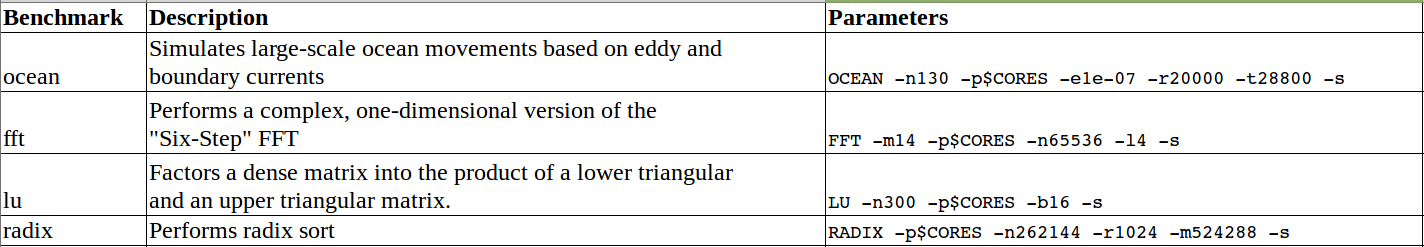
\includegraphics[scale=0.3]{../images/splash2.png}
    \caption{The specific SPLASH-2 benchmarks used}
    \label{fig:splash2_benchmarks}
\end{figure*}

\begin{figure*}
    \centering
    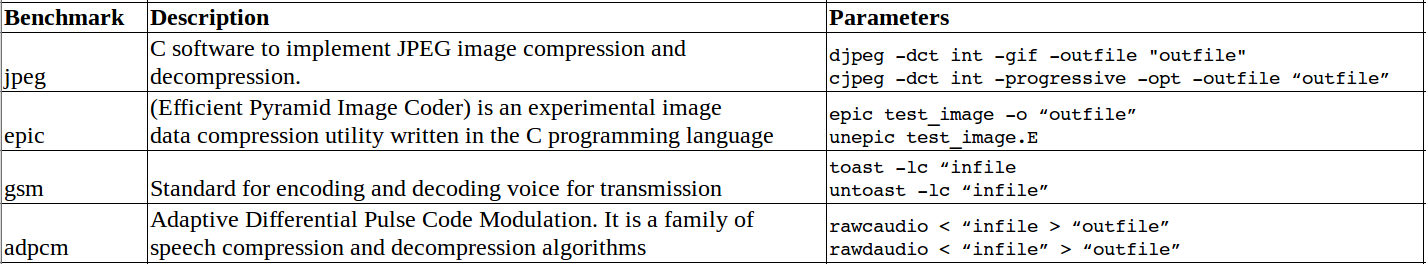
\includegraphics[scale=0.3]{../images/mb2.png}
    \caption{The specific MediaBench II benchmarks used}
    \label{fig:mb2_benchmarks}
\end{figure*}
For simulation of a dynamic processor, we needed two types of benchmarks. One which would be representative of highly parallelized workloads and one reflecting serial execution. The parallel benchmark we used was SPLASH-2 \cite{splash2}. SPLASH-2 is a suite of benchmarks intended to evaluate the performance of multiprocessor systems. For a serial benchmark suite, we chose to use MediaBench II \cite{mb2}. A suite of compression and decompression multimedia algorithms. The programs selected from each benchmark were intended to accurately reflect typical mobile device usage. Figures \ref{fig:splash2_benchmarks} and \ref{fib:mb2_benchmarks} detail the exact benchmarks used.

\subsection{Procedure}
When we initially began the project we planned on using gem5's SE mode for simplicity. However, due to the parallel nature of SPLASH-2 a multi-threading library is required. Because SE mode does not emulate a full operating system, there was no OS-level threading library such as pthreads. As a result, we finally decided to use full system mode. This provided us with access to Linux's full threading library allowing us to simulate the multi-threaded applications. Using full system mode had the additional benefit of providing extremely accurate results because the benchmarks are actually running in a Linux operating system, similar to our application space.

At this point, it was necessary to determine what CPU types and ISAs would be tested in order to simulate a dynamic processor. We initially planned on using either x86 or ARM as the underlying ISA. However, we soon found that only the AtomicSimple CPU model was supported by gem5 full system mode for these ISAs. gem5 provides much more complete support for the ALPHA ISA. ALPHA is a 64-bit RISC ISA representative of a simply architected general processor. Using this ISA as our building block we were able to develop benchmarks to represent a serial and a parallel machine. Our serial system used the O3 CPU model to simulate a modern out of order processor. Our parallel system was comprised of multiple TimingSimple CPU models. Originally, we had intended to use the InOrder model, however it was not available. Even though the TimingSimple CPU type was not a standard in-order pipeline, an array of the single cycle cores out performed the out-of-order processor on most parallel benchmarks. Thus, we felt the loss in accuracy was negligible.

In order to efficiently run tests, we developed scripts to boot a Linux kernel in FS mode and run through each of our benchmarks. At the completion of each benchmark the timing statistics would be written out to file. A script was then developed capable of parsing the output file and produce a CSV file containing the statistics for each benchmark. The Linux boot process became an advantage in our setup. Spanning 2.4 trillion instructions, we could be confident that all our caches would be warmed up after the boot process was complete. Furthermore, gem5's built-in stats-dump tool allowed us to run serial and parallel benchmarks one after the other without shutting the system down. This meant that the cache state before each benchmark was exactly the cache state at the end of the previous benchmark; thus, the initial cache miss latencies were embedded into our timing results.

Once we had the timing results for the serial and parallel models, we synthesized the results together to get the timing performance for a dynamic core. Of course, there is some latency associated with switching from a serial configuration to a dynamic configuration. Though we did not implement a dynamic core, we did theorize potential methods for a datapath. In particular, we were drawn to the idea of using muxes to run external inputs into the execution units of several cores. Based on this, it seemed appropriate that an advanced interconnect network would be required. Most multicore and system on a chip (SoC) devices use a crossbar network, but the crossbar is hardly scalable. Instead, many bleeding-edge devices use network-on-chip (NoC) structures that are based off of crossbar interconnects, but optimized for scalability and power dissapation. Thus, we selected a switching latency of 0.991 ns based on research in the field of NoCs \cite{lee}.

Furthermore, in order to study the problems surrounding a dynamic processor, we tackled two optimization issues. First, we chose a single serial program and a single parallel program to make up a single ``chunk'' of mixed code. We then look run time for 512 chunks put together. Then, the size of the serial and parallel portion in a chunk were doubled, so that each chunk is twice as large as it was before. However, we now only use 256 chunks in the test, so that the overall number of instructions remains constant. Repeating this process of doubling the size of a serial chunk and a parllel chunk while halving the number of chunks in the program, we are able to get results for the number of switches for maximum performance between serial and parallel portions within a fixed code segment. Secondly, we recognized that as the number of cores in the parallel model increases, the critical path of the serial model increases. Thus, the frequency should scale down for the serial model. Based on simple geometry (Pythagorean's theorem), we assume that the frequency will scale on the order of $1 / \sqrt{n}$. Thus, we obtained results for the serial model with scaled frequencies to see if there is a drop-off in performance.
